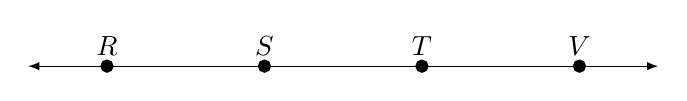
\begin{tikzpicture} 
\draw[>=latex,<->](0,0)--(8,0); 

 
\draw[thick, fill=black] (1,0) circle (.07cm) node[above]{$R$}; 
\draw[thick, fill=black] (3,0) circle (.07cm) node[above]{$S$}; 
\draw[thick, fill=black] (5,0) circle (.07cm) node[above]{$T$}; 
\draw[thick, fill=black] (7,0) circle (.07cm) node[above]{$V$}; 
\end{tikzpicture} 

Points \textit{R, S, T,} and \textit{V} lie on the real number line as shown below. The coordinate of \textit{S} is 0, $\overline{\textit{RT}}$ and is 20 units long, $\overline{\textit{SV}}$ and is 15 units long, and $\overline{\textit{RV}}$ and is 32 units long. What is the coordinate of \textit{T}?  

\ifsat
	\begin{enumerate}[label=\Alph*)]
		\item  $-1$ 
		\item  $1$ 
		\item  $3$ %
		\item  $14$ 
	\end{enumerate}
\else
\fi

\ifacteven
	\begin{enumerate}[label=\textbf{\Alph*.},itemsep=\fill,align=left]
		\setcounter{enumii}{5}
		\item   $-2$
		\item  $-1$ 
		\item  $1$ 
		\addtocounter{enumii}{1}
		\item  $3$ %
		\item  $14$ 
	\end{enumerate}
\else
\fi

\ifactodd
	\begin{enumerate}[label=\textbf{\Alph*.},itemsep=\fill,align=left]
		\item   $-2$
		\item  $-1$ 
		\item  $1$ 
		\item  $3$ %
		\item  $14$ 
	\end{enumerate}
\else
\fi

\ifgridin
  $3$ %
		
\else
\fi

